\chapter{Referencial Teórico}
\vspace{-2.5 cm}

Este Capítulo busca explanar os principais conceitos relacionados ao tema. 

\section{Arquitetura baseada em comportamento}

Um dos desafios que surgem em arquiteturas comportamentais é justamente a
seleção de ações tendo como base um conjunto de comportamentos
\cite{Livro_Mataric}. Duas maneiras tradicionais de fazer isso são: arbitragem e
fusão. Na arbitragem, seleciona-se apenas um dos comportamentos por vez,
enquanto que na fusão, os comportamentos operam em paralelo e suas saídas são
combinadas. Um esquema dos dois modelos pode ser visto na Figura \ref{fig:arbfus}. 

\tikzset{%
    block/.style={scale = 1.1, draw, fill=white, rectangle, 
            minimum height=2em, minimum width=3em},
    input/.style={inner sep=0pt},       
    output/.style={inner sep=0pt},      
    sum/.style = {scale = 1.1, draw, fill=white, circle, minimum size=2mm, node
    distance=1.5cm, inner sep=0pt},
    pinstyle/.style = {scale = 1.1, pin edge={to-,thin,black}}
}

\begin{figure}[h]%
    \caption{Arbitragem e fusão de comportamentos}%
    \label{fig:subfig2}%
    \centering
    
    \begin{subfigure}[t]{0.5\textwidth}%
	\centering
    
    %\resizebox{0.1\linewidth}{!}{
\begin{tikzpicture}[scale = 1.1, auto, node distance=2cm, on grid, >=latex']%
	\node[block] (C1) {Comportamento 1};
	\node[block, below = 1.6cm of C1] (C2) {Comportamento 2};
	\node[block, below = 1.6cm of C2] (C3) {Comportamento 3};
	\node[input, left = 2.5cm of C3] (int) {};
	\node[input, below = 1cm of int] (input) {};
	
	\node[right = 2.5cm of C2, inner sep = 0.2 cm] (sum) {};
	\node[right = 2.72cm of C2, inner sep = 0] (sum1int) {};
	\filldraw (sum1int) circle (0.8pt);
	\node[right = 2.3cm of C2, inner sep = 0] (sum2int) {};
	\node[above = 0.2cm of sum2int, inner sep = 0] (sum2) {};
	\node[output, right = 1cm of sum] (atu) {};
	 
	\coordinate[left = 2.5cm of C1, inner sep = 0pt] (lC1) {};
	\coordinate[left = 2.5cm of C2, inner sep = 0] (lC2) {};
	\coordinate[left = 2.5cm of C3, inner sep = 0] (lC3) {};
	
	\draw [draw,->] (sum) node[below right] {Atuadores} --
	(atu);
	
	\draw [draw,-] (input) node[above right] {Sensores} --
	(lC1);
	\draw [->] (lC1) -- (C1); 
	\draw [->] (lC2) -- (C2);
	\draw [->] (lC3) -- (C3);
	
	\draw [->] (C1) -| node[]{} node[near end] {} (sum);
	\draw [->] (C2) -- (sum);
	\draw [->] (C3) -| node[]{} node[near end] {} (sum);
	
	\draw [-, very thick] (sum1int) -- (sum2);
	
\end{tikzpicture}%    
    %}
    
    \label{fig:subfig1}%
	\caption{Arbitragem}%
	\end{subfigure}%
    ~
    \begin{subfigure}[t]{0.5\textwidth}%
	\centering
	%\resizebox{0.5\linewidth}{!}{
\begin{tikzpicture}[auto, node distance=2cm, on grid,
>=latex']%
	\node[block] (C1) {Comportamento 1};
	\node[block, below = 1.6cm of C1] (C2) {Comportamento 2};
	\node[block, below = 1.6cm of C2] (C3) {Comportamento 3};
	\node[input, left = 2.5cm of C3] (int) {};
	\node[input, below = 1cm of int] (input) {};
	
	\node[sum, right = 2.5cm of C2] (sum) {+};
	\node[output, right = 1cm of sum] (atu) {};
	 
	\coordinate[left = 2.5cm of C1, inner sep = 0pt] (lC1) {};
	\coordinate[left = 2.5cm of C2, inner sep = 0] (lC2) {};
	\coordinate[left = 2.5cm of C3, inner sep = 0] (lC3) {};
	
	\draw [draw,->] (sum) node[below right] {Atuadores} --
	(atu);
	
	\draw [draw,-] (input) node[above right] {Sensores} --
	(lC1);
	\draw [->] (lC1) -- (C1); 
	\draw [->] (lC2) -- (C2);
	\draw [->] (lC3) -- (C3);
	
	\draw [->] (C1) -| node[]{} node[near end] {} (sum);
	\draw [->] (C2) -- (sum);
	\draw [->] (C3) -| node[]{} node[near end] {} (sum);
	
\end{tikzpicture}%    
%}
	\caption{Fusão}%
	\end{subfigure}%
	
	\textbf{Fonte: baseado em \citeonline{Livro_Mataric}, p. 167.}
    \label{fig:arbfus}%
\end{figure}

%\begin{tikzpicture}[auto, node distance=2cm, on grid, >=latex']

%\node[input] (input) {};
%\node[input, above = of input] (input1) {};
%\node [sum, right = of input] (sum) {};
%\node [block, right = of sum] (controller) {$K(s)$};
%\node [sum, right = of controller] (sum1) {};
%\node [block, right = of sum1] (filterinv) {$H^{-1}(s)$};
%\node [block, right = 2.5cm of filterinv] (system) {$G(s)$};
%\node [output, right = of system] (output) {};
%\node [output, above = of output] (output1) {};
%\node [block, above = of controller] (delay) {$D(s)$};
%\node [sum, below = of sum1] (sum2) {};
%\node [block] (filter) at (sum2-|filterinv) {$H(s)$};

%\draw [draw,->] (input) node[above right] {$s_{i-1}$} -- (sum);
%\draw [->] (sum) -- node {$e_{i}$} (controller);
%\draw [->] (controller) -- node {} (sum1);
%\draw [->] (sum1) -- node[name=xi] {$\xi_{i}$} (filterinv);
%\draw [->] (filterinv) -- node[name=u, pos=.3] {$u_{i}$} (system);
%\draw [->] (system) -- (output) node [name=q, above left] {$q_{i}$};

%\draw [->] ([xshift=-5mm]q.south) |- (filter);
%\draw [->] (filter) -- node {} (sum2);
%\draw [draw,<-] (sum2) -- ++(90:.6cm) node[above]{$L_i+r_i$};

%\draw [->] (sum2) -| node[pos=0.99, right] {$-$} 
%    node [pos=.25, above] {$\tilde{s}_i$} (sum);

%\draw [draw,->] (input1) node[above right] (ui-1) {$u_{i-1}$} -- (delay);
%\draw [->] (delay) -| node[] {} 
%    node [near end] {} (sum1);

%\draw [->] (u.east|-system) |-  
%    (output1) node[above left] (ui) {$u_i$};

%\node[text=red, above left= 5mm and 6mm of ui.west] (veh) {vehicle $i$};
%\draw[red, dashed]
% (veh.east)-|(ui.west)|-([yshift=-3mm]filter.south)-|(ui-1.east)|-(veh.west);

%\end{tikzpicture}

\subsection{Comportamentos como campos potenciais}

Uma forma de definir comportamentos é por meio de campos potenciais, onde o
vetor gradiente determina uma direção de referência para o sistema de controle
\cite{book:arkin, art:wallfollowing}. Como exemplo, uma possível escolha para um
comportamento de ``Ir Para Objetivo'' é dado na Equação \ref{eq:vetGTG},
retratada na Figura \ref{fig:campovet}.a (R = 1). Já o comportamento ``Evitar
Obstáculo'' (pontual) pode ser descrito pela Equação \ref{eq:vetAO}, retratada
na Figura \ref{fig:campovet}.b (R = 0 e S = 1). Nas equações, S é uma esfera de
influência, R é uma distância crítica, $\mathbf{\hat{u}}_{ipo}$ e
$\mathbf{\hat{u}}_{eo}$ são vetores unitários que apontam, respectivamente,
para o objetivo e na direção oposta ao obstáculo.
\begin{equation}
	\label{eq:vetGTG}
	V(x,y) = \left \{ \begin{matrix} \mathbf{\hat{u}}_{ipo} &, \ para\ d \geq R \\
	\ \frac{d}{R}\ \mathbf{\hat{u}}_{ipo} &,\ para\ d < R \end{matrix} \right.
\end{equation}
\begin{equation}
	\label{eq:vetAO}
	V(x,y) = \left \{ \begin{matrix} [0\quad0]^{T} &, \ para\ d > S \\
	\ \frac{S-d}{S-R}\ \mathbf{\hat{u}}_{eo} &\quad \ \ \ ,\ para\ R < d \leq S \\
	\mathbf{\hat{u}}_{eo} &,\ para\ d \leq R \end{matrix} \right.
\end{equation} 

\begin{figure}[h]%
    \caption{Comportamentos definidos por campos potenciais}%
    %\label{fig:subfig2}%
    \centering
    
    \begin{subfigure}[t]{0.5\textwidth}%
	\centering
    
    %\resizebox{0.1\linewidth}{!}{
\begin{tikzpicture}[auto, node distance=2cm, on grid, >=latex']%
\begin{axis}[view={0}{90}, axis equal image]
	\addplot3[darkgray, domain=-2:2, y domain=-2:2, 
		quiver={
			u={-x}, v={-y},
			scale arrows=0.2}, ->,samples=21,
			y filter/.append
			code={\pgfmathparse{(sqrt(x^2+y^2)>1.8)||(sqrt(x^2+y^2)<0.1||(sqrt(x^2+y^2)>1))
			? nan : y}}] {0};
			
	\addplot3[darkgray, domain=-2:2, y domain=-2:2, 
		quiver={
			u={-x/(sqrt(x^2+y^2))}, v={-y/(sqrt(x^2+y^2)},
			scale arrows=0.2}, ->,samples=21,
			y filter/.append
			code={\pgfmathparse{(sqrt(x^2+y^2)>1.8)||(sqrt(x^2+y^2)<0.1||(sqrt(x^2+y^2)<=1))
			? nan : y}}] {0};
			
	\addplot3[gray, domain=-1.905:1.905, y domain=-1.905:1.905, 
		quiver={
			u={-x}, v={-y},
			scale arrows=0.2}, ->,samples=20,
			y filter/.append
			code={\pgfmathparse{(sqrt(x^2+y^2)>1.8)||(sqrt(x^2+y^2)<0.1)||(sqrt(x^2+y^2)>1)
			? nan : y}}] {0};
			
	\addplot3[gray, domain=-1.905:1.905, y domain=-1.905:1.905, 
		quiver={
			u={-x/(sqrt(x^2+y^2))}, v={-y/(sqrt(x^2+y^2))},
			scale arrows=0.2}, ->,samples=20,
			y filter/.append
			code={\pgfmathparse{(sqrt(x^2+y^2)>1.8)||(sqrt(x^2+y^2)<0.1)||(sqrt(x^2+y^2)<=1)
			? nan : y}}] {0};
			
\end{axis}
\end{tikzpicture}%    
    %}
    
    %\label{fig:subfig1}%
	\caption{Comportamento ``Ir Para Objetivo''}%
	\end{subfigure}%
    ~
    \begin{subfigure}[t]{0.5\textwidth}%
	\centering
	%\resizebox{0.5\linewidth}{!}{
\begin{tikzpicture}[auto, node distance=2cm, on grid,
>=latex']%
\begin{axis}[view={0}{90}, axis equal image]
\addplot3[darkgray, domain=-2:2, y domain=-2:2, 
		quiver={
			u={-x/2 + x/(sqrt(x^2+y^2))}, v={-y/2 + y/(sqrt(x^2+y^2))}, scale
			arrows=0.25}, ->,samples=21, 
			y filter/.append
			code={\pgfmathparse{(sqrt(x^2+y^2)>1.8)||(sqrt(x^2+y^2)<0.1) ? nan : y}}] {0};

\addplot3[gray, domain=-1.905:1.905, y domain=-1.905:1.905, 
		quiver={
			u={-x/2 + x/(sqrt(x^2+y^2))}, v={-y/2 + y/(sqrt(x^2+y^2))},
			scale arrows=0.25}, ->,samples=20,
			y filter/.append
			code={\pgfmathparse{(sqrt(x^2+y^2)>1.8)||(sqrt(x^2+y^2)<0.1) ? nan : y}}]
			{0};

\end{axis}
\end{tikzpicture}%    
%}
	\caption{Comportamento ``Evitar Obstáculo''}%
	\end{subfigure}%
	
	\textbf{Fonte: baseado em \citeonline{book:arkin}, p. 146 e 148}
    \label{fig:campovet}%
\end{figure}

Em um robô real, cada sensor é associado a uma distância até um obstáculo
(mesmo que infinitamente distante) e, consequentemente, a um vetor definido pelo
comportamento ``Evitar Obstáculo''. Uma combinação linear entre estes vetores
cria um obstáculo virtual pontual a partir de obstáculos não pontuais
\cite{art:wallfollowing}. 

Vetores associados a comportamentos distintos podem ser combinados (linearmente)
a fim de obter uma ação intermediária (Fusão, retratada na Figura
\ref{fig:arbfus}.b), ou suas magnitudes são comparadas de modo que o
``vencedor'' assume controle pleno (Arbitragem, retratada na Figura
\ref{fig:arbfus}.a). 

A estratégia de utilizar campos potenciais tem suas particularidades, já que
podem existir mínimos locais, o que leva o robô a parar antes de chegar ao
objetivo. Para resolver este problema, deve-se, ou estabelecer um campo
potencial sem mínimos locais, ou desenvolver métodos para escapar deles
\cite{art:wallfollowing}. \citeonline{art:wallfollowing} apresentam uma solução
do segundo tipo, ao definir um comportamento ``Seguidor de Parede''.

%\begin{figure}[h]%
    \caption{Mínimos Locais ao combinar comportamentos}%
    %\label{fig:subfig2}%
    \centering    
    %\resizebox{0.1\linewidth}{!}{
\begin{tikzpicture}[auto, node distance=2cm, on grid, >=latex']%
\begin{axis}[view={0}{90}, axis equal image]
	\addplot3[darkgray, domain=-2:2, y domain=-2:2, 
		quiver={
			u={-x}, v={-y},
			scale arrows=0.2}, ->,samples=21,
			y filter/.append
			code={\pgfmathparse{(sqrt(x^2+y^2)>1.8)||(sqrt(x^2+y^2)<0.1||(sqrt(x^2+y^2)>1))
			? nan : y}}] {0};
			
	\addplot3[darkgray, domain=-2:2, y domain=-2:2, 
		quiver={
			u={-x/(sqrt(x^2+y^2))}, v={-y/(sqrt(x^2+y^2)},
			scale arrows=0.2}, ->,samples=21,
			y filter/.append
			code={\pgfmathparse{(sqrt(x^2+y^2)>1.8)||(sqrt(x^2+y^2)<0.1||(sqrt(x^2+y^2)<=1))
			? nan : y}}] {0};
			
	\addplot3[gray, domain=-1.905:1.905, y domain=-1.905:1.905, 
		quiver={
			u={-x}, v={-y},
			scale arrows=0.2}, ->,samples=20,
			y filter/.append
			code={\pgfmathparse{(sqrt(x^2+y^2)>1.8)||(sqrt(x^2+y^2)<0.1)||(sqrt(x^2+y^2)>1)
			? nan : y}}] {0};
			
	\addplot3[gray, domain=-1.905:1.905, y domain=-1.905:1.905, 
		quiver={
			u={-x/(sqrt(x^2+y^2))}, v={-y/(sqrt(x^2+y^2))},
			scale arrows=0.2}, ->,samples=20,
			y filter/.append
			code={\pgfmathparse{(sqrt(x^2+y^2)>1.8)||(sqrt(x^2+y^2)<0.1)||(sqrt(x^2+y^2)<=1)
			? nan : y}}] {0};
			
			
\addplot3[darkgray, domain=-2:2, y domain=-2:2, 
		quiver={
			u={-x/2 + x/(sqrt(x^2+y^2))}, v={-y/2 + y/(sqrt(x^2+y^2))}, scale
			arrows=0.25}, ->,samples=21, 
			y filter/.append
			code={\pgfmathparse{(sqrt(x^2+y^2)>1.8)||(sqrt(x^2+y^2)<0.1) ? nan : y}}] {0};

\addplot3[gray, domain=-1.905:1.905, y domain=-1.905:1.905, 
		quiver={
			u={-x/2 + x/(sqrt(x^2+y^2))}, v={-y/2 + y/(sqrt(x^2+y^2))},
			scale arrows=0.25}, ->,samples=20,
			y filter/.append
			code={\pgfmathparse{(sqrt(x^2+y^2)>1.8)||(sqrt(x^2+y^2)<0.1) ? nan : y}}]
			{0};
\end{axis}
\end{tikzpicture}%    
%}	

	\textbf{Fonte: baseado em \citeonline{book:arkin}, p. 146 e 148}
    \label{fig:MinimoLocal}%
\end{figure}

\section{Modelagem}

Nesta seção serão levantados os modelos cinemáticos para o robô móvel de
acionamento diferencial e uniciclo. A seguir, será feita uma relação entre os
dois, que permitirá realizar o controle do robô diferencial a partir do
uniciclo, tornando mais simples o projeto. Os esquemas dos dois modelos pode ser
visto na Figura \ref{fig:modelo}.

%\begin{tikzpicture}[x=0.5cm,y=0.5cm,z=0.3cm,>=stealth]
% The axes

\newcommand{\coordsystwo}[1]{
	\draw[->] (xyz cs:x=0) -- (xyz cs:x=1.5) node[right] {$\hat{X}_{#1}$};
	\draw[->] (xyz cs:y=0) -- (xyz cs:y=1.5) node[above] {$\hat{Y}_{#1}$};
	% The thin ticks
	%\foreach \coo in {-13,-12,...,13}
	%{
	%  \draw (\coo,-1.5pt) -- (\coo,1.5pt);
	%  \draw (-1.5pt,\coo) -- (1.5pt,\coo);
	%  \draw (xyz cs:y=-0.15pt,z=\coo) -- (xyz cs:y=0.15pt,z=\coo);
	%}
	
	% The thick ticks
	%\foreach \coo in {-10,-5,5,10}
	%{
	%\draw[thick] (\coo,-3pt) -- (\coo,3pt) node[below=6pt] {\coo};
	%\draw[thick] (-3pt,\coo) -- (3pt,\coo) node[left=6pt] {\coo};
	%\draw[thick] (xyz cs:y=-0.3pt,z=\coo) -- (xyz cs:y=0.3pt,z=\coo)
	% node[below=8pt] {\coo}; }
	
	% Dashed lines for the points P, Q
	%\draw[dashed] 
	%\draw[dashed] (u) -- (v);
	%\draw[dashed] (-5,7) -- (-5,0) -- (w);
	%\draw[dashed] (3,0) |- (0,5);
	
	% Dots and labels for P, Q
	%\node[fill,circle,inner sep=1.5pt,label={left:$Q(-5,-5,7)$}] at (0,0) {};
	%\node[fill,circle,inner sep=1.5pt,label={above:$P(3,0,5)$}] at (3,5) {};
	% The origin

	% Ponto na origem do sistema de coordenadas
	\node[fill,circle,inner sep=1pt] at (0,0) {};
	
	% Seta para indicar Sistema de coordenadas {X}
	%\node[align=center] at (2,-2) (ori) {\{#1\}};
	%\draw[->,help lines,shorten >=3pt] (ori) .. controls (0.6,-1.3) and (1,-1) ..
	%(0,0,0);
}

\newcommand{\robodiff}{
	% Linhas de baixo, lat esq e dir
	\draw[-, inner sep = 0] (-0.65,-0.75) -- (0.65,-0.75);
	\draw[-, inner sep = 0] (-0.75,-0.65) -- (-0.75,0.5);
	\draw[-, inner sep = 0] (0.75,-0.65) -- (0.75,0.5);
	
	% bordas de baixo
	\draw[-, inner sep = 0] (-0.65,-0.75) -- (-0.75,-0.65);
	\draw[-, inner sep = 0] (0.65,-0.75) -- (0.75,-0.65);
	
	% Retas de cima
	\def\UserL{\fpeval{1.3/(2*cosd(45)+1)}}
	\draw[-, inner sep = 0] (-0.75,0.5) -- (\fpeval{-0.75+\UserL*cosd(45)},
	\fpeval{0.5+\UserL*sind(45)});
	
	\draw[-, inner sep = 0] (0.75,0.5) -- (\fpeval{0.75-\UserL*cosd(45)},
	\fpeval{0.5+\UserL*sind(45)});
	
	\draw[-, inner sep = 0]
	(\fpeval{-0.75+\UserL*cosd(45)},\fpeval{0.5+\UserL*sind(45)}) -- (\fpeval{0.75-\UserL*cosd(45)},
	\fpeval{0.5+\UserL*sind(45)});
	
	% Bola de rolamento
	\filldraw (0,0.65) circle (1.5pt);
	\draw (0,0.65) circle (3pt);
	
	% Desenhar rodas
	\begin{scope}[shift={(-0.75,-0.65)},rotate = 90]
		\draw[rounded corners=2pt] (0,0) rectangle ++(0.8,0.2);
	\end{scope}
	\begin{scope}[shift={(0.75,-0.65)},rotate = 90]
		\draw[rounded corners=2pt] (0,0) rectangle ++(0.8,-0.2);
	\end{scope}
	
	%\draw[dashed, -, inner sep = 0] (-0.75,-0.25) -- (0.75,-0.25);
	
	% Medida R
	\draw[-, inner sep = 0] (+1.2,-0.3) -- ++(0,0.5) node[right] at (+1.4,-0.15)
	{R};
	\draw[-, inner sep = 0] (+1.25,-0.25) -- ++(-0.1,0);
	\draw[-, inner sep = 0] (+1.25,0.15) -- ++(-0.1,0);
	% Medida L
	\draw[-, inner sep = 0] (-0.8,-1) -- (0.8,-1) node[below] at (-0.1,-1.2){L};
	\draw[-, inner sep = 0] (-0.75,-1.05) -- ++(0,0.1);
	\draw[-, inner sep = 0] (0.75,-1.05) -- ++(0,0.1);	
}

\newcommand{\robodiffinercial}{
	\begin{tikzpicture}[scale = 1.5]
		\coordsystwo{I}
		%\draw[-{latex}, shorten >=1.5pt] (0,0) -- (2,2) node[above] at
		%(2.1,0.6){$^{A}Q_{B_{origem}}$};
		% Translação
		\begin{scope}[shift={(2, 2)}]
			%\coordsys{A'}
			% Rotação
			\draw[->] (0.3,0) arc (0:60:0.3);
			\draw[-] (0,0) -- (0.4,0);
			\node at (0.5,0.3) {$\phi$};
			
			% Po 
			\node[color = gray] at (0.1,-0.25) {$P_o$};
			
			\begin{scope}[rotate=60]
				% Ponto Pr
				\node[fill,circle,inner sep=1pt] at (0.6,0) {};
			 	\node[color = gray] at (0.65,0.25) {$P_r$};
			 	\node[color = gray] at (0.3,0.15) {$l$};
			
				\coordsystwo{R}
				\begin{scope}[shift={(0.25,0)},rotate = -90]
					\robodiff
				\end{scope}
				% Flecha até P
				%\draw[-{latex}, shorten >=1.5pt] (0,0) -- (1,2.4) node[right] {$^{B}P$};
				% Ponto em P
				%\node[fill,circle,inner sep=1pt] at (1,2.4) {}; 
				% Definir ponto para desenhar reta
				%\node[align=center,inner sep=0pt] at (1,2.4) (Ponto) {};
			\end{scope}	
		\end{scope}
	% Ponto de {A} para {B}
	%\draw[dashed, -{latex}, shorten >=1pt] (0,0) -- (Ponto) node[above] at (1.5,
	%1.8) {$^{A}P$};
	\end{tikzpicture}
}

\newcommand{\robouniciclo}{
	\begin{scope}[rotate = 90]
	\begin{scope}[shift={(-0.6, -0.15)}]
		\draw[rounded corners=2pt] (0,0) rectangle ++(1.2,0.3);
	\end{scope}
	\end{scope}
}

\newcommand{\robounicicloinercial}{
	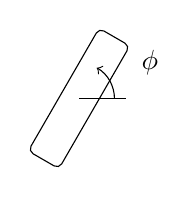
\begin{tikzpicture}[scale = 1.5]
		\coordsystwo{I}
		%\draw[-{latex}, shorten >=1.5pt] (0,0) -- (2,2) node[above] at
		%(2.1,0.6){$^{A}Q_{B_{origem}}$};
		% Translação
		\begin{scope}[shift={(2, 2)}]
			%\coordsys{A'}
			% Rotação
			\draw[->] (0.3,0) arc (0:60:0.3);
			\draw[-] (0,0) -- (0.4,0);
			\node at (0.6,0.3) {$\phi$};
			
			\begin{scope}[rotate=60]
				\coordsystwo{R}
				\begin{scope}[rotate = -90]
					\robouniciclo
				\end{scope}
				% Flecha até P
				%\draw[-{latex}, shorten >=1.5pt] (0,0) -- (1,2.4) node[right] {$^{B}P$};
				% Ponto em P
				%\node[fill,circle,inner sep=1pt] at (1,2.4) {}; 
				% Definir ponto para desenhar reta
				%\node[align=center,inner sep=0pt] at (1,2.4) (Ponto) {};
			\end{scope}	
		\end{scope}
	% Ponto de {A} para {B}
	%\draw[dashed, -{latex}, shorten >=1pt] (0,0) -- (Ponto) node[above] at (1.5,
	%1.8) {$^{A}P$};
	\end{tikzpicture}
}

\begin{figure}[h]
\centering
\caption{Modelos uniciclo e diferencial} \label{fig:modelo}
	\begin{subfigure}[t]{0.5\textwidth}%
		\centering
		\robounicicloinercial
		\label{fig:uniciclo}%
		\caption{Uniciclo}%
		\end{subfigure}%
    	~
    	\begin{subfigure}[t]{0.5\textwidth}%
		\centering
		\robodiffinercial
		\label{fig:diff}%
		\caption{Diferencial}%
		\end{subfigure}%
		
		\textbf{Fonte: baseado em \citeonline{Livro_Siegwart}, p. 49 e 54.}
\end{figure}

%\begin{tikzpicture}[x=0.5cm,y=0.5cm,z=0.3cm,>=stealth]

	\subsection{Modelo cinemático do uniciclo}

O modelo uniciclo representa uma única roda que se movimenta em uma
superfície sem deslizamento. Considera-se que existe acesso direto às
velocidades linear e angular. 

O modelo cinemático pode ser visto na Equação
\ref{eq:uniciclo} \cite{lavalle2006planning}. A Equação \ref{eq:unimat}
representa o uniciclo na forma matricial \cite{Livro_Siegwart}.
\begin{equation}
	\label{eq:uniciclo}
	\left \{ \begin{matrix} \dot{x} &= v\cos{\phi} \\ \dot{y} &= v\sin{\phi} \\
	\dot{\phi} &= \omega \end{matrix} \right.
\end{equation}
\begin{equation}
	\label{eq:unimat}
	\mleft[ 
	\begin{array}{c c}
	\dot{x} \\ \dot{y} \\ \dot{\phi}
	\end{array}
	\mright] = \mleft[
	\begin{matrix}
		  \cos{\phi} & 0 \\
		  \sin{\phi} & 0 \\
		  0 & 1 \\
	\end{matrix}
	\mright] \mleft[ 
	\begin{array}{c c}
	v \\ \omega
	\end{array}
	\mright]
\end{equation}

	\subsection{Modelo cinemático do robô móvel de acionamento diferencial}	

Neste modelo (Equação \ref{eq:diff}), são consideradas como entradas as
velocidades angulares das rodas esquerda e direita \cite{lavalle2006planning}. 
\begin{equation}
	\label{eq:diff}
	\left \{ \begin{matrix} \dot{x} = \frac{R}{2}(\omega_l +
	\omega_r)\cos{\phi}
	\\
	\dot{y} = \frac{R}{2}(\omega_l +
	\omega_r)\sin{\phi}
	\\
	\dot{\phi} = \frac{R}{L}(\omega_r -
	\omega_l) \end{matrix} \right.
\end{equation}

O robô móvel de acionamento diferencial, arquitetura usada neste trabalho, é
cinematicamente equivalente ao uniciclo \cite{tese:franca}. Isso pode ser
mostrado igualando $\dot{x}$, $\dot{y}$ e $\dot{\phi}$ das Equações
\ref{eq:uniciclo} e \ref{eq:diff}. Resolvendo para $\omega_l$ e $\omega_r$,
tem-se a igualdade da Equação \ref{eq:vw_to_diff}.
\begin{equation}
	\label{eq:vw_to_diff}
	\begin{matrix}
	\omega_l = \frac{2v - L\omega}{2R} 
	\\
	\omega_r = \frac{2v + L\omega}{2R}
	\end{matrix}
\end{equation}

Essa equivalência entre modelos é possível pois eles não consideram a dinâmica
do sistema \cite{lavalle2006planning}.

	%\subsection{Linearização do modelo}
	%\subsection{Odometria}
	
%%%%%%%%%%%%%%%%%%%%%%%%%%%%%%%%%%%%%%%%%
%				Controle				%
%%%%%%%%%%%%%%%%%%%%%%%%%%%%%%%%%%%%%%%%%	
\section{Considerações para o controle de robôs móveis}

O sistema uniciclo tem duas restrições ditas não holonômicas, o que significa
que não podem ser integradas para obter uma restrição geométrica
\cite{Oriolo2013}.
Na Equação \ref{eq:restricoes}, a primeira se refere à ausência de deslizamento
lateral, enquanto a segunda é relativa à condição de rotação pura (ausência de
deslizamento no sentido do vetor velocidade) \cite[pg.
955]{book:AdvancedDynamics}.
\begin{equation}
	\label{eq:restricoes}
	\begin{matrix}
	\dot{x}\sin{\phi} - \dot{y}\cos{\phi} = 0 
	\\
	\dot{x}\cos{\phi} + \dot{y}\sin{\phi} = v
	\end{matrix}
\end{equation}

Dois tipos de problemas em controle de robôs móveis podem ser explicitados:
estabilização em um determinado estado (configuração) e seguir trajetória
(\textit{tracking}). Pela própria natureza do sistema não holonômico, o primeiro
problema é considerado mais difícil \cite{tese:franca}.

No caso da estabilização, o teorema de Brockett afirma que, para sistemas
subatuados, com menos entradas que variáveis de estado, o sistema não pode ser
estabilizado assintoticamente (exponencialmente) usando leis de controle por
realimentação de estado contínuas e invariantes no tempo
\cite{artigo:ASTOLFI1995661, inbook:Ravi_Mumbai}.
Para solucionar esse problema, técnicas de controle não linear têm sido
exploradas, envolvendo controladores descontínuos e/ou variantes no tempo
\cite{tese:franca}.  

O fato do robô movel ser de estado completamente controlável
apesar de subatuado é devido à presença de restrições não holonômicas
\cite{Oriolo2013}.

Para o problema de seguir trajetória (\textit{tracking}), o objetivo é seguir
uma curva parametrizada em função do tempo \cite{art:Manuel}. 

Em \citeonline{art:Magnus_PMPC}, uma técnica é explorada a fim de tratar o
modelo diferencial pelo modelo de integrador-único (ponto controlado por
velocidade, ou, $\mathbf{\dot{x}} = \mathbf{u}$). Os autores utilizam como
referência um ponto deslocado em relação ao ponto no centro entre as duas rodas.
A Figura \ref{fig:modelo}.b indica a posição deste ponto ($P_r$) e a Equação
\ref{eq:Pr} mostra os valores de x e y para a nova referência. Derivando e
substituindo $\dot{x}$, $\dot{y}$ e $\dot{\phi}$ da Equação \ref{eq:uniciclo},
obtem-se a Equação \ref{eq:PrDeriv}.
\begin{equation}
	\label{eq:Pr}
	\left \{ \begin{matrix} x' = x_o + l\cos{\phi}
	\\
	y' = y_o + l\sin{\phi}
	\end{matrix} \right.
\end{equation}
\begin{equation}
	\label{eq:PrDeriv}
	\left \{ \begin{matrix} \dot{x'} = \dot{x_o} - \dot{\phi}l\sin{\phi} =
	v\cos{\phi} - l\omega\sin{\phi}
	\\
	\dot{y'} = \dot{y_o} + \dot{\phi}l\cos{\phi} = v\sin{\phi} + l\omega\cos{\phi}
	\end{matrix} \right.
\end{equation}

A Equação \ref{eq:single_integrator} é idêntica à \ref{eq:PrDeriv}, porém, na
forma matricial. Sua inversa estabelece um mapeamento direto entre as entradas
$[\dot{x}\ \dot{y}]^T$ do modelo de integrador-único para as entradas do modelo
uniciclo (Equação \ref{eq:si_inv_uni}), ou modelo diferencial (Equação
\ref{eq:si_inv_diff}).
\begin{equation}
	\label{eq:single_integrator}
	\mleft[ 
	\begin{array}{c c}
	\dot{x'} \\ \dot{y'}
	\end{array}
	\mright] = \mleft[
	\begin{matrix}
		  \cos{\phi} & -\sin{\phi} \\
		  \sin{\phi} & \cos{\phi} \\
	\end{matrix}
	\mright] \mleft[
	\begin{matrix}
		  1 & 0 \\
		  0 & l \\
	\end{matrix}
	\mright] \mleft[ 
	\begin{array}{c c}
	v \\ \omega
	\end{array}
	\mright]
\end{equation}
\begin{equation}
	\label{eq:si_inv_uni}
	\mleft[ 
	\begin{array}{c c}
	v \\ \omega
	\end{array}
	\mright] = \mleft[
	\begin{matrix}
		  1 & 0 \\
		  0 & \frac{1}{l} \\
	\end{matrix}
	\mright] \mleft[
	\begin{matrix}
		  \cos{\phi} & \sin{\phi} \\
		  -\sin{\phi} & \cos{\phi} \\
	\end{matrix}
	\mright] \mleft[ 
	\begin{array}{c c}
	\dot{x'} \\ \dot{y'}
	\end{array}
	\mright]
\end{equation}
\begin{equation}
	\label{eq:si_inv_diff}
	\mleft[ 
	\begin{array}{c c}
	\omega_l \\ \omega_r
	\end{array}
	\mright] = \mleft[
	\begin{matrix}
		  \frac{1}{R} & \frac{-L}{2R} \\
		  \frac{1}{R} & \frac{L}{2R} \\
	\end{matrix}
	\mright] \mleft[
	\begin{matrix}
		  1 & 0 \\
		  0 & \frac{1}{l} \\
	\end{matrix}
	\mright] \mleft[
	\begin{matrix}
		  \cos{\phi} & \sin{\phi} \\
		  -\sin{\phi} & \cos{\phi} \\
	\end{matrix}
	\mright] \mleft[ 
	\begin{array}{c c}
	\dot{x'} \\ \dot{y'}
	\end{array}
	\mright]
\end{equation}

Pelo que pode ser verificado em \citeonline{art:Magnus_PMPC}, os modelos
uniciclo e de integrador-único não são equivalentes, já que $l$ não pode tender
a zero. Um controle de modelo preditivo é estabelecido para ajustar $l$ a fim de
obter uma resposta que sacrifique o mínimo possível em precisão e
manobrabilidade, comparando com uma escolha estática de parâmetro ($l =
\sqrt{\frac{1-\alpha}{\alpha}\frac{Lv_{max}}{R}}$, com $\alpha = 0,99$). 

Esta técnica, também chamada ``\textit{look-ahead}'', é utilizada, com
modificações, em alguns trabalhos como passo intermediário antes de realizar uma
linearização por realimentação \cite{art:feedlin_lookahead, art:novel}. Em
\citeonline{art:feedlin_lookahead} é mostrado que o modelo dinâmico não pode ser
linearizado por realimentação entrada-estado. A linearização por realimentação
entrada-saída estática só é possível adotando esta nova referência.

Apesar de em \citeonline{art:feedlin_lookahead} a dinâmica do sistema ser
considerada, em \citeonline{art:novel} é dito que um modelo cinemático pode ser
usado. Ao considerar a dinâmica (primeiro trabalho) uma realimentação é
definida de forma a compensar não linearidades do sistema, a fim de tratá-lo
como um modelo de duplo integrador ($\mathbf{\ddot{x}} = \mathbf{u}$). A partir
disso, o sistema pode ser controlado por técnicas de controle linear. 

Para o modelo cinemático deste trabalho, a definição de um campo potêncial não é
tão conveniente, já que o negativo do gradiente associado especifica
força, de modo que a aceleração é obtida considerando massa
\cite{art:wallfollowing, book:HallidayDaMassa}. Em \citeonline{art:vectorfield},
o campo vetorial definido indica velocidades. Os vetores velocidade calculados
podem ser usados como entrada do modelo de integrador único.

Apesar do modelo não ser controlável por técnicas lineares, é possível utilizar 
controle PID para seguir ângulo, com a limitação de não ter controle sobre 
velocidades linear ou angular. Para aplicações onde a convergência não tem
restrições temporais significativas, controle angular é suficiente e será 
utilizado no caso deste trabalho.

% Campo potencial X Campo vetorial de velocidades.

%%%%%%%%%%%%%%%%%%%%%%%%%%%%%%%%%%%%%%%%%
%				DES						%
%%%%%%%%%%%%%%%%%%%%%%%%%%%%%%%%%%%%%%%%%	
\section{Sistemas a eventos discretos}

Um Sistema a Eventos Discretos (SED) pode ser caracterizado como um sistema
dinâmico, cujos estados são discretos, sendo que transições entre estes estados ocorrem
a partir da detecção de eventos assíncronos \cite{book:SED}. Um evento pode ser
definido como um estímulo que provoca transições instantâneas de estado. Na
ausência de eventos, o sistema permanece no mesmo estado \cite{man:Cury}.

Um SED pode ser modelado usando o formalismo presente em teoria de computação:
linguagens regulares e autômatos finitos. O autômato finito determinístico é uma
tupla $M=(Q,\Sigma,\delta,q,F)$ formada por um conjunto de estados ($Q$), um conjunto
de símbolos ($\Sigma$), uma função de transição ($\delta$), um estado inicial
($q$), e um conjunto de estados finais ($F$, que é subconjunto de $Q$). \cite{book:SED,
book:TeoriaComp}.

O conjunto de eventos admissíveis em um SED é o alfabeto de uma linguagem e um
conjunto de eventos sucessivos seriam palavras desta linguagem. O autômato
representa uma linguagem formal. Uma forma de representar o autômato é por meio
de um diagrama de transição de estado. Um exemplo pode ser visto na Figura
\ref{fig:diagrama}.

\tikzset{%
    block/.style={draw, fill=white, rectangle, 
            minimum height=2em, minimum width=3em},
    input/.style={inner sep=0pt},       
    output/.style={inner sep=0pt},      
    sum/.style = {draw, fill=white, circle, minimum size=2mm, node
    distance=1.5cm, inner sep=0pt},
    pinstyle/.style = {pin edge={to-,thin,black}}
}

\begin{figure}[ht]
    \caption{Diagrama de Transição de Estado}%
    \label{fig:diagrama}%
    \centering
        
\begin{tikzpicture}[scale = 1.2, ->,auto,node distance =4 cm and 5cm ,on grid,
>=latex',
state/.style ={scale = 1.2, circle, draw, minimum width =0.7cm},
finalstate/.style ={scale = 1.2, circle, draw, minimum width =0.7cm}]

	\node[finalstate, double, double distance=1pt, outer sep = 1pt] (x) {$x$};
	\node[state, right = 3.4cm of x] (y) {$y$};
	\node[finalstate, double, double distance = 1pt, outer sep = 1pt, below right
	= 2.5cm of x] (z) {$z$};
	
	\path[->] (x) edge node[below left] {$g$} (z);
	\path[->] (z) edge node[below right] {$a,g$} (y);
	\path[->] (y) edge node[above] {$a$} (x);
	
	\draw (x) to [out=60,in=120,looseness=6] node[above] {$a$} (x);
	\draw (y) to [out=60,in=120,looseness=6] node[above] {$b$} (y);
	\draw (z) to [out=240,in=300,looseness=6] node[below] {$b$} (z);
	
	% Input
	\coordinate[left = 1cm of x, inner sep = 0pt] (input) {};
	\path[->] (input) edge (x);
\end{tikzpicture}%    
	
	\textbf{Fonte: baseado em \citeonline{book:SED}, p. 60.}
    \label{fig:diagrama}%
\end{figure}

O SED possui um comportamento, ou dinâmica, que pretende-se controlar, já que
algumas cadeias de eventos aceitas pela linguagem podem não ser desejadas. A
estrutura ou agente responsável pelo controle é chamado supervisor, que interage
com a planta capturando eventos ocorridos (apenas aqueles que são
observáveis) e atuando de forma a permitir ou suprimir eventos passíveis de
ocorrência \cite{book:SED}. Um esquema desta interação pode ser visto na Figura
\ref{fig:supmalhafechada}.

\tikzset{%
    block/.style={scale = 1.2, draw, fill=white, rectangle, 
            minimum height=2em, minimum width=3em},
    input/.style={inner sep=0pt},       
    output/.style={inner sep=0pt},      
    sum/.style = {scale = 1.2, draw, fill=white, circle, minimum size=2mm, node
    distance=1.5cm, inner sep=0pt},
    pinstyle/.style = {scale = 1.2, pin edge={to-,thin,black}}
}

\begin{figure}[h]%
    \caption{SED em malha fechada}%
    \centering
    
\begin{tikzpicture}[scale = 1.2, auto, node distance=2cm, on grid,
>=latex']%
	\node[block] (P) {Planta};
	\node[block, below = 1.8cm of P] (S) {Supervisor};
	
	\coordinate[left = 2cm of S, inner sep = 0pt] (int1) {};
	\coordinate[right = 2cm of P, inner sep = 0pt] (int2) {};
	
	\draw [->] (P) -| (int2) node[below right] {Eventos Observados} |- (S);
	\draw [->] (S) -| (int1) node[above left] {Eventos Desabilitados} |- (P);
	
	%node[above] {$a$}
\end{tikzpicture}%    
	
	\textbf{Fonte: baseado em \citeonline{man:Cury}, p. 49.}
    \label{fig:supmalhafechada}%
\end{figure}



\subsection{Autômatos temporizados com guardas}

Uma representação mais completa é o autômato temporizado com guardas, que possui
um conjunto de variáveis contínuas e em função do tempo denominadas
\textit{clocks}, cuja dinâmica é linear. O temporizador pode ser usado para
estabelecer condições que provocam transições. Durante essas transições, a
variável temporizada pode sofrer \textit{reset} (onde o valor 0 é atribuido)
\cite{book:SED}.

Transições temporizadas são tuplas da forma (guardas; eventos;
\textit{reset}), onde ``guardas'' é um conjunto de condições em variáveis
do tipo \textit{clock} que devem ser atendidas para ocorrência de transição,
os eventos são componentes já definidos e \textit{reset} especifica um conjunto
de variáveis do tipo \textit{clock} às quais deve ser atribuído valor 0.
Quando o conjunto ``guardas'' é vazio $\emptyset$, considera-se valor
lógico verdadeiro e quando o conjunto \textit{reset} é vazio, nenhuma variável
\textit{clock} sofre atribuição de valor 0 \cite{book:SED}. Dois exemplo de
diagramas de transição são mostrados na Figura \ref{fig:ATG}. 

\tikzset{%
    block/.style={draw, fill=white, rectangle, 
            minimum height=2em, minimum width=3em},
    input/.style={inner sep=0pt},       
    output/.style={inner sep=0pt},      
    sum/.style = {draw, fill=white, circle, minimum size=2mm, node distance=1.5cm, inner sep=0pt},
    pinstyle/.style = {pin edge={to-,thin,black}}
}

\newcommand{\diagum}{
\begin{tikzpicture}[scale = 1.1,->,auto ,node distance =4 cm and 5cm , on grid,
>=latex' ,
state/.style ={scale = 1.1, circle, draw, minimum width =0.7cm},
finalstate/.style ={scale = 1.1, circle, draw, minimum width =0.7cm}]

	\node[state] (a) {0};
	\node[state, above right = 2.5cm of a] (b) {1};
	\node[state, below right = 2.5cm of b] (c) {2};
	\node[state, below left = 2.5cm of c] (d) {3};
	
	\path[->] (a) edge node[above left] {$\emptyset; a; c_1$} (b);
	\path[->] (b) edge node[above right] {$0<c_1<1; a; c_1$} (c);
	\path[->] (c) edge node[below right] {$c_1<1; b; \emptyset$} (d);
	\draw (b) to [out=120,in=60,looseness=6] node[above] {$c_1\geq1;a;c_1$} (b);
	
	% Input
	\coordinate[left = 1cm of a, inner sep = 0pt] (input) {};
	\path[->] (input) edge (a);
\end{tikzpicture}%
}

\newcommand{\diagdois}{
\begin{tikzpicture}[->,auto ,node distance =4 cm and 5cm ,on grid ,
>=latex' ,
state/.style ={scale = 1.1, circle, draw, minimum width =0.7cm},
finalstate/.style ={scale = 1.1, circle, draw, minimum width =0.7cm}]

	\node[state] (a) {0};
	\node[state, above right = 2.5cm of a] (b) {1};
	\node[state, below right = 2.5cm of b, align = center] (c) {2 \\ $c_1<1$};
	\node[state, below left = 2.5cm of c] (d) {3};
	
	\path[->] (a) edge node[above left] {$\emptyset; a; c_1$} (b);
	\path[->] (b) edge node[above right] {$0<c_1<1; a; c_1$} (c);
	\path[->] (c) edge node[below right] {$\emptyset; b; \emptyset$} (d);
	\draw (b) to [out=120,in=60,looseness=6] node[above] {$c_1\geq1;a;c_1$} (b);
	
	% Input
	\coordinate[left = 1cm of a, inner sep = 0pt] (input) {};
	\path[->] (input) edge (a);	
\end{tikzpicture}%
}

% Figura
\begin{figure}[h]
\centering
\caption{Exemplos de diagramas de transição para autômatos temporizados com
guarda} 
	\label{fig:ATG}
	\begin{subfigure}[t]{0.5\textwidth}%
		\centering
		\diagum%
		\label{fig:guardadiag1}%
		\caption{Exemplo 1}%
		\end{subfigure}%
    	~
    	\begin{subfigure}[t]{0.5\textwidth}%
		\centering
		\diagdois%
		\label{fig:guardadiag2}%
		\caption{Exemplo 2}%
		\end{subfigure}%
		
		\textbf{Fonte: baseado em \citeonline{book:SED}, p. 301.}
\end{figure}

Em casos nos quais a condição de guarda deixa de ser válida, como, por exemplo,
quando no estado 2 da Figura \ref{fig:ATG}.a, $c_1$ se torna maior ou igual a 1, ocorre
\textit{deadlock} por tempo (\textit{timelock}). Quando é necessário forçar a
ocorrência de um evento para evitar \textit{timelock}, modela-se como na Figura
\ref{fig:ATG}.b. A condição associada a um estado é chamada Invariante
\cite{book:SED}.

%Dois exemplo de diagramas de transição são mostrados na Figura
%\ref{fig:ATG}. \textit{Deadlocks} por tempo podem acontecer em casos onde a
%condição de guarda deixa de ser válida, como por exemplo quando, no estado 2 da
%Figura \ref{fig:ATG}.a, $c_1$ se torna maior ou igual a 1. Quando é necessário
%forçar a ocorrência de um evento para evitar \textit{deadlock}, modela-se como
%na Figura \ref{fig:ATG}.b \cite{book:SED}.

Por fim, o autômato pode ser representado como uma tupla (Q, E, C, Tra, Inv,
$q_0$), onde Q é um conjunto de estados, E é um conjunto de eventos, C é um
conjunto de temporizadores (variáveis contínuas), ``Tra'' é um conjunto de
transições temporizadas, ``Inv'' é um conjunto de invariantes e $q_0$ é o
estado inicial \cite{book:SED}.

\section{Sistemas híbridos}

Sistemas híbridos são formados quando Sistemas Dinâmicos de Variável
Contínua (SDVC) e Sistemas a Eventos Discretos (SED) funcionam de maneira
conjunta. Neste caso, controladores de variável contínua são abstraídos
por um SED. Transições de estado provocam transições ou ``chaveamento'' entre
controladores \cite{book:SED}. A Figura \ref{fig:supervisorio} mostra o esquema
da arquitetura de controle de um sistema híbrido.

\tikzset{%
    block/.style={scale = 1.3,draw, fill=white, rectangle, 
            minimum height=2em, minimum width=3em},
    input/.style={inner sep=0pt},       
    output/.style={inner sep=0pt},      
    sum/.style = {scale = 1.3,draw, fill=white, circle, minimum size=2mm, node
    distance=1.5cm, inner sep=0pt},
    pinstyle/.style = {scale = 1.3,pin edge={to-,thin,black}}
}

\begin{figure}[ht]%
    \caption{Controlador Híbrido}%
    \label{fig:subfig2}%
    \centering
    
\begin{tikzpicture}[scale = 1.3,auto, node distance=2cm, on grid, >=latex']%
	\node[block] (C1) {Controlador Supervisório};
	\node[block, below = 2.7cm of C1] (C2) {Interface};
	\node[block, below = 2.7cm of C2] (C3) {Controlador de Variável Contínua};
	\node[block, below = 2.7cm of C3] (C4) {Sistema};
	
	\coordinate[left = 0.5cm of C1.south, inner sep = 0pt] (c1vai) {};
	\coordinate[right = 0.5cm of C1.south, inner sep = 0pt] (c1vem) {};
	\coordinate[right = 0.5cm of C2.north, inner sep = 0pt] (c2vai) {};
	\coordinate[left = 0.5cm of C2.north, inner sep = 0pt] (c2vem) {};
	\draw [draw,->] (c1vai.south) -- (c2vem.north);
	\draw [draw,->] (c2vai.north) -- (c1vem.south);
	
	\node[below = 0.7cm of C1.south, inner sep = 0pt] (comand) {};
	\node (com1) {};
	\node[left = 1.6cm of comand, inner sep = 0pt] (com) {Comandos};
	\node[right = 2.5cm of comand, inner sep = 0pt] (ev) {Eventos Observáveis};
	
	%\node[below = 2cm of C1, inner sep = 0 cm] (C1) {Comandos};
	%\node[below right = 1.5cm of C1, inner sep = 0.2 cm] () {Eventos Observáveis};
	
	\coordinate[left = 0.5cm of C2.south, inner sep = 0pt] (c2vaibelow) {};
	\coordinate[right = 0.5cm of C2.south, inner sep = 0pt] (c2vembelow) {};
	\coordinate[right = 0.5cm of C3.north, inner sep = 0pt] (c3vai) {};
	\coordinate[left = 0.5cm of C3.north, inner sep = 0pt] (c3vem) {};
	\draw [draw,->] (c2vaibelow.south) -- (c3vem.north);
	\draw [draw,->] (c3vai.north) -- (c2vembelow.south);
	
	\coordinate[left = 1.4cm of C3.south, inner sep = 0pt] (c3vaibelow) {};
	\coordinate[right = 1.4cm of C3.south, inner sep = 0pt] (c3vembelow) {};
	\coordinate[above = 0.15cm of C4.east, inner sep = 0pt] (c41vai) {};
	\coordinate[above = 0.15cm of C4.west, inner sep = 0pt] (c41vem) {};
	
	\draw [->] (c3vaibelow) |- (c41vem);
	\draw [->] (c41vai) -| (c3vembelow);
	
	\coordinate[below = 0.15cm of C4.east, inner sep = 0pt] (c42vai) {};
	\coordinate[below = 0.15cm of C4.west, inner sep = 0pt] (c42vem) {};
	\coordinate[left = 3cm of c42vem, inner sep = 0pt] (int1) {};
	\coordinate[right = 3cm of c42vai, inner sep = 0pt] (int2) {};
	
	\draw [->] (C2.west) -| (int1) |- (c42vem);
	\draw [->] (c42vai) -| (int2) |- (C2.east);
\end{tikzpicture}%    
	
	\textbf{Fonte: baseado em \citeonline{book:SED}, p. 43.}
    \label{fig:supervisorio}%
\end{figure} 

Neste sentido, é necessário introduzir o conceito de autômatos híbridos. Ao
invés de estados discretos, os estados do sistema são dados por
$(q,\mathbf{x})$, com $q \in Q$, onde $Q$ é um conjunto de estados discretos e
$\mathbf{x} \in X$, onde $X$ é um conjunto de estados contínuos. O estado $q$
determina o modo de operação do sistema. O autômato híbrido é, portanto, uma extensão do
autômato temporizado com guardas, já que as funções dos temporizadores
(lineares) podem ser substituídas por funções arbitrárias \cite{book:SED}.

Esse novo autômato pode ser representado pela tupla $G_h = (Q, X,
E, U, f, \phi, Inv, guard, \rho, q_0, \mathbf{x_0})$, onde Q é um conjunto de
estados discretos, X é um conjunto de variáveis contínuas (o espaço de estados
X $\subseteq \mathbb{R}^n$), E é um conjunto de eventos, U é um conjunto de
entradas controláveis (U $\subseteq \mathbb{R}^m$), $f$ é um campo vetorial
($f: Q \times X \times U \rightarrow X$), $\phi$ é uma função de transição de
estados discretos ($\phi: Q \times X \times E \rightarrow Q$), ``Inv'' é um
conjunto de invariantes, ou domínio ($Inv \subseteq Q \times X$), ``guard'' é um
conjunto de condições de guarda ($guard \subseteq Q \times Q \times X$), $\rho$
é uma função \textit{reset} ($\rho: Q \times Q \times X \times E \rightarrow
X$) cujo objetivo é alterar \textbf{x} quando ocorre mudança de modo (q), $q_0$
é o estado discreto inicial (modo de operação) e $\mathbf{x_0}$ é o estado
contínuo inicial \cite[pg. 316]{book:SED}.

Em robótica móvel, autômatos fornecem um meio de implementar a arbitragem
requisitada pela arquitetura baseada em comportamentos, onde cada modo de
operação corresponde a um comportamento. Porém, o uso de autômatos híbridos
traz uma particularidade potencialmente problemática: o comportamento de
Zenão, no qual, teoricamente, transições infinitas de modo ocorrem em tempo finito, o que
bloqueia a passagem de tempo \cite{art:Magnus_Behavior}.

Isso ocorre quando o campo vetorial descontínuo subjacente a um sistema híbrido
converge para uma superfície de separação entre modos, o que é chamado de
deslize. Essa limitação do autômato, no ambiente real, provoca oscilações, já
que mudanças de controladores ocorrem em curto espaço de tempo. Uma possível
solução é por meio do processo de regularização, que na prática adiciona um
estado de forma a implementar uma ``dinâmica de deslize'' sobre a fronteira que
separa comportamentos \cite{art:Magnus_Behavior}. Este conceito está ilustrado
na Figura \ref{fig:Sliding}.

\tikzset{%
    block/.style={draw, fill=white, rectangle, 
            minimum height=2em, minimum width=3em},
    input/.style={inner sep=0pt},       
    output/.style={inner sep=0pt},      
    sum/.style = {draw, fill=white, circle, minimum size=2mm, node distance=1.5cm, inner sep=0pt},
    pinstyle/.style = {pin edge={to-,thin,black}}
}

\newcommand{\sliding}{
\begin{tikzpicture}[scale = 1.1,->,auto ,node distance =4 cm and 5cm ,on grid ,
>=latex' ,
state/.style ={scale = 1.1,circle, draw, minimum width =0.7cm},
finalstate/.style ={scale = 1.1,circle, draw, minimum width =0.7cm}]

	\coordinate (supa) {};
	\coordinate[right = 4cm of supa] (supb) {};
	\draw[-,dashed] (supa) to [out=45,in=135] (supb);
	
	\coordinate[above right = 2cm of supa, inner sep = 0pt] (in1) {};
	\coordinate[below = 1.25cm of in1, inner sep = 0pt] (in2) {};
	\coordinate[below right = 0.835cm of in1] (dest) {};
	\path[->] (in1) edge node[above right] {$f_1$} (dest);
	\path[->] (in2) edge node[below right] {$f_2$}(dest);
	
	\coordinate[right = 0.7cm of dest, inner sep = 0pt] (dest2) {};
	\path[->] (dest) edge node[above right] {$f_S$}(dest2);
	
	\node[above = 0.5cm of supb] (b) {$\sigma = 0$};
\end{tikzpicture}%
}

\newcommand{\diagreg}{
\begin{tikzpicture}[scale = 1.1,->,auto ,node distance =4 cm and 5cm ,on grid ,
>=latex' ,
state/.style ={scale = 1.1,circle, draw, minimum width =0.7cm},
finalstate/.style ={scale = 1.1,circle, draw, minimum width =0.7cm}]
	
	\node[ellipse, draw] (f1) {$\dot{x} = f_1$};
	\node[ellipse, draw, right = 3.5cm of f1] (f2) {$\dot{x} = f_2$};
	
	\draw (f1) to [out=30,in=150] node[above] {$\sigma \leq 0$} (f2);
	\draw (f2) to [out=210,in=330] node[below] {$\sigma \geq 0$} (f1);
	
	\node[ellipse, draw, below = 2.8cm of f1] (f1l) {$\dot{x} = f_1$};
	\node[ellipse, draw, right = 2.5cm of f1l] (fsl) {$\dot{x} = f_S$};
	\node[ellipse, draw, right = 2.5cm of fsl] (f2l) {$\dot{x} = f_2$};
	
	\draw (f1l) to [out=30,in=150] node[above] {$\sigma \leq 0$} (fsl);
	\draw (fsl) to [out=210,in=330] node[below] {$\sigma > 0$} (f1l);
	\draw (fsl) to [out=30,in=150] node[above] {$\sigma < 0$} (f2l);
	\draw (f2l) to [out=210,in=330] node[below] {$\sigma \geq 0$} (fsl);
	
	%(f1) {$\dot{x} = f_1$};
	
	%\node[state] (a) {0};
	%\node[state, above right = 2.5cm of a] (b) {1};
	%\node[state, below right = 2.5cm of b, align = center] (c) {2 \\ $c_1<1$};
	%\node[state, below left = 2.5cm of c] (d) {3};
	
	%\path[->] (a) edge node[above left] {$\emptyset; a; c_1$} (b);
	%\path[->] (b) edge node[above right] {$0<c_1<1; a; c_1$} (c);
	%\path[->] (c) edge node[below right] {$\emptyset; b; \emptyset$} (d);
	%\draw (b) to [out=120,in=60,looseness=6] node[above] {$c_1\geq1;a;c_1$} (b);
	
	% Input
	%\coordinate[left = 1cm of a, inner sep = 0pt] (input) {};
	%\path[->] (input) edge (a);	
\end{tikzpicture}%
}

% Figura
\begin{figure}[h]
\centering
\caption{Modo deslizante e diagramas de transição} 
	\label{fig:Sliding}
	\begin{subfigure}[t]{0.5\textwidth}%
		\centering
		\raisebox{15mm}
		\sliding%
		\label{fig:sliding2}%
		\caption{Solução deslizante}%
		\end{subfigure}%
    	~
    	\begin{subfigure}[t]{0.5\textwidth}%
		\centering
		\diagreg%
		\label{fig:diagreg}%
		\caption{Diagramas de transição original e regularizado}%
		\end{subfigure}%
		
		\textbf{Fonte: baseado em \citeonline{art:Magnus_Behavior}}
\end{figure}

O termo ``comportamento de Zenão'' faz alusão ao filósofo grego Zenão de
Eleia, conhecido pelos seus famosos paradoxos \cite{art:Magnus_Behavior}. 

%%%%%%%%%%%%%%%%%%%%%%%%%%%%%%%%%%%%%%%%%
%			Lógica Fuzzy				%
%%%%%%%%%%%%%%%%%%%%%%%%%%%%%%%%%%%%%%%%%
\section{Lógica \textit{Fuzzy} em Controle}

Em certas circunstâncias, a lógica Booleana pode não ser suficiente
para descrever conhecimentos qualitativos com precisão. Como exemplo, ao
determinar como ``alto'' todo indivíduo com altura maior que 1,70 metros,
pessoas com 1,71 ou 2,00 metros seriam consideradas igualmente altas.
A lógica \textit{Fuzzy} acrescenta a informação de ``pertinência'', que atribui um
``grau de certeza" de um valor (neste exemplo, altura) em relação à classe
avaliada (categoria ``alto'') \cite{fuzzylilly}.

Sistemas \textit{Fuzzy} tem por objetivo mesclar aspectos exatos com
conhecimentos imprecisos que caracterizam o pensamento humano. Deste modo,
aspectos qualitativos de um problema, ou conhecimento especializado, são
mapeados e utilizados em um sistema \textit{Fuzzy} \cite{fuzzylilly}. Um
diagrama de blocos de um controlador \textit{Fuzzy} e seus componentes atuando
em um sistema pode ser visto na Figura \ref{fig:ContFuzzy}.

\tikzset{%
    block/.style={draw, fill=white, rectangle, 
            minimum height=2em, minimum width=3em, align=center},
    input/.style={inner sep=0pt},       
    output/.style={inner sep=0pt},      
    sum/.style = {draw, fill=white, circle, minimum size=2mm, node distance=1.5cm, inner sep=0pt},
    pinstyle/.style = {pin edge={to-,thin,black}}
}

\begin{figure}[h]%
    \caption{Diagrama de blocos para um sistema com controlador \textit{Fuzzy}}%
    \centering
    
\begin{tikzpicture}[auto, node distance=2cm, on grid,
>=latex']%
	\node[block] (Fat) {Fatores \\ de escala, \\ normalização};
	\node[block, right = 3.2 cm of Fat] (Fuz) {Fuzzyficação};
	\node[block, right = 2.9 cm of Fuz] (Inf) {Mecanismo \\ de Inferência};
	\node[block, right = 3.1 cm of Inf] (Defuz) {Defuzzyficação};
		
	\node[block, right = 2.6 cm of Defuz] (Planta) {Planta};
	
	\node[block, above = 2 cm of Fuz] (kno) {Base de \\ conhecimento};
	\node[block, above = 2 cm of Inf] (Base) {Base de \\ regras};
	\node[block, below = 2 cm of Defuz] (Sensor) {Sensores};
	\node[block, below = 2 cm of Inf] (outfat) {Fatores de \\ escala de
	saída, \\ normalização};
	
	\coordinate[left = 2cm of Fat] (input) {};
	\coordinate[right = 1.2cm of Planta] (output) {};
	
	\draw[->] (input) node[above] {Entrada} -- (Fat);
	\draw[<->] (kno) -- (Fuz);
	\draw[<->] (Base) -- (Inf);
	\draw[->] (Fuz) -- (Inf);
	\draw[->] (Inf) -- (Defuz);
	\draw[->] (Defuz) -- (Planta);
	\draw[->] (Sensor) -- (outfat);
	\draw[->] (Planta) -- (output) node[above] {Saída};
	
	\draw [->] (output) -- (output)+(-0.3cm,0) |- (Sensor);
	
	\coordinate[above = 0.15cm of Fuz.west] (infuz1) {};
	\coordinate[below = 0.15cm of Fuz.west] (infuz2) {};
	\coordinate[above = 0.15cm of Fat.east] (int1) {};
	\coordinate[left = 0.5cm of infuz2] (int2) {};
	
	\draw [->] (outfat) -| (int2) |- (infuz2);
	\draw [->] (int1) -- (infuz1);
	
	% Quadrado - Controlador Fuzzy
	%\draw[gray,thick,dashed] ($(Fuz.north west)+(-0.2,0.5)$)  rectangle
	%($(Defuz.south east)+(0.2,-0.5)$);
	%\node[above = 1.15 cm of Defuz] (escrita) {Controlador \textit{Fuzzy}};
	
	\draw[gray,thick,dashed] ($(kno.north west)+(-0.2,0.3)$)  rectangle
	($(Defuz.south east)+(0.2,-0.3)$);
	\node[above = 2.55 cm of Defuz] (escrita) {Controlador \textit{Fuzzy}};
	
\end{tikzpicture}%    
	
	\textbf{Fonte: baseado em \citeonline{fuzzy_ross}, p. 442 e
	\citeonline{fuzzylilly}, p.	29.} \label{fig:ContFuzzy}%
\end{figure}

Os sistemas \textit{Fuzzy}, de acordo com \citeonline{fuzzy_ross}, são
úteis em contextos onde é necessário lidar com sistemas muito complexos,
compreendidos parcialmente, além de casos nos quais soluções rápidas
são desejadas, mesmo que aproximadas. 

Já \citeonline{fuzzylilly} afirma que problemas não lineares, de difícil
solução por controle clássico, são exemplos de situações nas quais sistemas
\textit{Fuzzy} podem ser utilizados. Entretando, o autor alerta que, por conta
do alto custo computacional desta solução, ela não é indicada para casos
envolvendo problemas lineares e invariantes no tempo, nos quais soluções
mais diretas estão disponíveis, por exemplo, controle PID e técnica de alocação
de pólos. 

\subsection{Conjuntos Fuzzy}

No exemplo dado anteriormente, uma proposição da lógica booleana foi usada para
definir um conjunto dos indivíduos ``altos''. Este conjunto (convencional) é
chamado ``crisp''. Em conjuntos \textit{Fuzzy}, associa-se a cada membro de
um conjunto um valor real entre 0 e 1 chamado ``grau de pertinência'', onde 0
representa exclusão absoluta, 1 representa pertinência total e qualquer valor
intermediário representa pertinência parcial \cite{fuzzylilly}. 

Os valores numéricos possíveis para altura são chamados ``universo de
discurso'', o valor ``alto'' é dito ser um ``valor linguístico'' associado a
``comprimento'', que é a variável linguística no exemplo dado. Para ilustrar o
conceito, funções de pertinência associadas à variável linguística ``altura''
podem ser vistas na Figura \ref{fig:conjfuzzy}, onde $\mu$ é o grau de
pertinência. Assim, valores de altura podem pertencer a mais de uma classe,
porém com diferentes graus de pertinência \cite{fuzzylilly}.

\tikzset{%
    block/.style={draw, fill=white, rectangle, 
            minimum height=2em, minimum width=3em},
    input/.style={inner sep=0pt},       
    output/.style={inner sep=0pt},      
    sum/.style = {draw, fill=white, circle, minimum size=2mm, node distance=1.5cm, inner sep=0pt},
    pinstyle/.style = {pin edge={to-,thin,black}}
}

\begin{figure}[ht]%
    \caption{Conjuntos \textit{Fuzzy} possíveis para a variável ``altura''}%
    \label{fig:conjfuzzy}%
    \centering
    
\begin{tikzpicture}[scale = 1, auto, node distance=2cm, on grid, >=latex']%
	\begin{axis}[xmin=0.9, xmax=2.1,ymax=1.1, samples=50, xlabel={Altura (m)},
	ylabel={$\mu$}]
	
		\addplot [thick, color=black] table {
			0 1
			1 1
			1.7 0
			3 0
		};
		
		\addplot [thick, color=black] table {
			0 0
			1.3 0
			1.6 1
			1.9 0
			3 0
		};
		
		\addplot [thick, color=black] table {
			0 0 
			1.4 0
			2 1
			3 1
		};
		
  		%\addplot[blue, ultra thick] (x,x/10);
  		%\addplot[red,  ultra thick] (x,x/10 + 1);
	\end{axis}
	\node[color=gray] at (1.3,5.2) {baixo};
	\node[color=gray] at (3.3,5.2) {médio};
	\node[color=gray] at (5.7,5.2) {alto};
	
	%\draw[smooth, samples=100,domain=0:2] plot(\x,{(\x)});
\end{tikzpicture}%
	
	\textbf{Fonte: baseado em \citeonline{fuzzylilly}, p. 32.}
    %\label{fig:conjfuzzy}%
\end{figure}


As definições conceituais em teoria de conjuntos são diferentes para conjuntos
\textit{Fuzzy}. As mais importantes, explicitadas em \citeonline{fuzzylilly},
estão reunidas a seguir, onde $\mu_1(x)$ e $\mu_2(x)$ são graus de pertinência
relacionados aos conjuntos \textit{Fuzzy} $M_1$ e $M_2$, respectivamente,
definidas para uma mesma variável $x$ no universo de discurso $\chi$.

\begin{itemize}
  \item Subconjunto: $M_1$ é subconjunto \textit{Fuzzy} de $M_2$ ($M_1
  \subseteq M_2$) se $\mu_1 \leq \mu_2$, $\forall x \in \chi$.
  
  \item Complemento: o complemento \textit{Fuzzy} de M ($\overline{M}$) é dado
  por $\mu_{\overline{M}}(x) = 1 - \mu_M (x)$.
  
  \item Intersecção (AND): 
  
  Pode ser usada qualquer função que cumpra os requisitos:  
  \begin{enumerate}
    \item Um elemento do universo não pode pertencer a dois conjuntos
    \textit{Fuzzy} com maior grau de pertinência que a cada conjunto
    individualmente.
    \item Se um elemento não pertence a um dos conjuntos, não pode pertencer à
    intersecção. 
    \item Se um elemento pertence aos dois conjuntos \textit{Fuzzy} com
    pertinência total, então pertence à intersecção com pertinência total. 
  \end{enumerate}

Duas funções que cumprem os requisitos são: $\mu_{M_1 \bigcap M_2}(x) =
min\{\mu_1(x),\mu_2(x): x \in \chi\}$ (função mínimo) e $\mu_{M_1 \bigcap
M_2}(x) = \{\mu_1(x)\mu_2(x): x \in \chi\}$ (produto algébrico).  
  
  \item União (OR):
  
  Pode ser usada qualquer função que cumpra os requisitos:
  \begin{enumerate}
    \item Um elemento do universo não pode pertencer à união de dois conjunto
    \textit{Fuzzy} com menor grau de pertinência que a cada conjunto
    individualmente.
    \item Se um elemento pertence a um dos conjuntos, então deve pertencer à
    união. 
    \item Se um elemento não pertence a nenhum dos dois conjuntos
    \textit{Fuzzy}, então não pertence à união.
  \end{enumerate}
  
Duas funções que cumprem o requisito são: $\mu_{M_1 \bigcup M_2}(x) =
max\{\mu_1(x),\mu_2(x): x \in \chi\}$ (função máximo) e $\mu_{M_1 \bigcup
M_2}(x) = \{\mu_1(x) + \mu_2(x) - \mu_1(x)\mu_2(x): x \in \chi\}$ (soma
algébrica).
\end{itemize}

Um exemplo das operações união e intersecção pode ser visto na figura
\ref{fig:ANDOR}.

\tikzset{%
    block/.style={draw, fill=white, rectangle, 
            minimum height=2em, minimum width=3em},
    input/.style={inner sep=0pt},       
    output/.style={inner sep=0pt},      
    sum/.style = {draw, fill=white, circle, minimum size=2mm, node distance=1.5cm, inner sep=0pt},
    pinstyle/.style = {pin edge={to-,thin,black}}
}

% Figura
\begin{figure}[ht]
\centering
\caption{Operações união e intersecção em conjuntos \textit{Fuzzy}} 
	\label{fig:ANDOR}
	\begin{subfigure}[t]{0.5\textwidth}%
		\centering
		
		%%%%%%%%%%%%%%%%%%%%%%%%%%%%%%%%%%%
		\begin{tikzpicture}[scale = 1, auto, node distance=2cm, on grid, >=latex']%
	\begin{axis}[xmax=38,ymax=1.1, samples=50]
	
		\addplot[color=gray] table {
			5 0
			15 1
			25 0
		};
		
		\addplot [color=gray] table {
			15 0
			25 1
			35 0
		};
		
		%% And - intersecção
		\addplot [thick, color=black] table {
			15 0
			20 0.5
			25 0
		};
  		%\addplot[blue, ultra thick] (x,x/10);
  		%\addplot[red,  ultra thick] (x,x/10 + 1);
	\end{axis}	
	%\draw[smooth, samples=100,domain=0:2] plot(\x,{(\x)});
\end{tikzpicture}%
		%%%%%%%%%%%%%%%%%%%%%%%%%%%%%%%%%%%

		\label{fig:exemploAnd}%
		\caption{Intersecção usando função ``min''}%
		\end{subfigure}%
    	~
    	\begin{subfigure}[t]{0.5\textwidth}%
		\centering
		%%%%%%%%%%%%%%%%%%%%%%%%%%%%%%%%%%%%%%%
		\begin{tikzpicture}[scale = 1, auto, node distance=2cm, on grid, >=latex']%
	\begin{axis}[xmax=38,ymax=1.1, samples=50]
	
		\addplot [color=gray] table {
			5 0
			15 1
			25 0
		};
		
		\addplot [color=gray] table {
			15 0
			25 1
			35 0
		};
		
		%% Or - União
		\addplot [thick, color=black] table {
			5 0
			15 1
			20 0.5
			25 1
			35 0
		};
  		%\addplot[blue, ultra thick] (x,x/10);
  		%\addplot[red,  ultra thick] (x,x/10 + 1);
	\end{axis}	
	%\draw[smooth, samples=100,domain=0:2] plot(\x,{(\x)});
\end{tikzpicture}%
		%%%%%%%%%%%%%%%%%%%%%%%%%%%%%%%%%%%%%%%
		\label{fig:exemploOr}%
		\caption{União usando função ``max''}%
		\end{subfigure}%
		
		\textbf{Fonte: baseado em \citeonline{fuzzylilly}, p. 20 e 21.}
\end{figure}
% Produto Cartesiano
% Conjuntos Fuzzy Singleton

\subsection{Componentes de um Sistema \textit{Fuzzy}}

Conhecimento qualitativo é utilizado para gerar regras do tipo ``Se P
então Q", que relacionam valores linguísticos de entrada com valores
linguísticos de saída. O conjunto de regras forma a ``Base de Regras'', que
pode ser vista como uma tabela de consulta, com número de dimensões igual
ao número de variáveis \cite{fuzzy_passino}.

	\subsubsection{Fuzzificação}
	
	O processo de associar variáveis numéricas a conjuntos fuzzy, a fim de obter
	valores linguísticos com seus respectivos valores de pertinência, é denominado
	Fuzzificação. A saída deste processo é o conjunto de graus de pertinência
	vinculados aos valores linguísticos definidos \cite{fuzzy_passino}.
	
	%Fuzzificação singleton
	\subsubsection{Mecanismo de Inferência}
	
	Ao final do processo de fuzzificação, a Base de Regras deve ser utilizada para
	encontrar saídas definidas por variáveis linguísticas. Contudo, apenas entradas
	associadas a graus de pertinência maiores que zero devem ser levados em
	consideração, a fim de obter um subconjunto de regras (ativas) a serem
	avaliadas \cite{fuzzy_passino}.
	
	Um conjunto de regras ativas e os respectivos graus de pertinência de suas
	premissas são utilizados para calcular funções de pertinência para cada regra.
	Como exemplo, dadas as regras $A \rightarrow C$ e $B \rightarrow D$, onde as
	premissas A e B possuem pertinências $\mu_A = 0,75$ e $\mu_B = 0,25$, e os
	consequentes C e D possuem funções de pertinência mostradas na Figura
	\ref{fig:FuzzyInferencia}.a. As Figuras \ref{fig:FuzzyInferencia}.b e
	\ref{fig:FuzzyInferencia}.c mostram funções de pertinência obtidas para as
	regras. As saídas destas regras são vistas como	recomendações que, apesar de
	conflitantes, podem ser combinadas de acordo com sua importância (pertinência)
	\cite{fuzzy_passino}.
	
	\tikzset{%
    block/.style={draw, fill=white, rectangle, 
            minimum height=2em, minimum width=3em},
    input/.style={inner sep=0pt},       
    output/.style={inner sep=0pt},      
    sum/.style = {draw, fill=white, circle, minimum size=2mm, node distance=1.5cm, inner sep=0pt},
    pinstyle/.style = {pin edge={to-,thin,black}}
}

% Figura
\begin{figure}[h]
\centering
\caption{Inferência em Lógica \textit{Fuzzy}}
	\label{fig:FuzzyInferencia}
	\begin{subfigure}[b]{0.33\textwidth}%
		\centering
%		\resizebox{\linewidth}{!}{
		%%%%%%%%%%%%%%%%%%%%%%%%%%%%%%%%%%%
		\begin{tikzpicture}[scale = 0.65, auto, node distance=2cm, on grid, >=latex']%
		\begin{axis}[xmax=38,ymax=1.1, samples=50]
	
		\addplot [thick, color=gray] table {
			5 0
			15 1
			25 0
		};
		
		\addplot [thick, color=gray] table {
			15 0
			25 1
			35 0
		};
		
		\node[] at (75,95) {C};
		\node[] at (225,95) {D};
  		%\addplot[blue, ultra thick] (x,x/10);
  		%\addplot[red,  ultra thick] (x,x/10 + 1);
	\end{axis}		
		%\draw[smooth, samples=100,domain=0:2] plot(\x,{(\x)});
		\end{tikzpicture}%
		%%%%%%%%%%%%%%%%%%%%%%%%%%%%%%%%%%%
		
		\label{fig:exemploAnd}%
		\caption{Funções de pertinência para C e D}%
		\end{subfigure}%
    	~
    	\begin{subfigure}[b]{0.33\textwidth}%
		\centering
		%%%%%%%%%%%%%%%%%%%%%%%%%%%%%%%%%%%%%%%
%		\resizebox{\linewidth}{!}{
		\begin{tikzpicture}[scale = 0.65, auto, node distance=2cm, on grid, >=latex']%
	\begin{axis}[xmax=38,ymax=1.1, samples=50]
	
		\addplot [color=gray] table {
			5 0
			15 1
			25 0
		};
		
		\addplot [thick, color=black] table {
			5 0
			12.5 0.75
			17.5 0.75
			25 0
		};
	\end{axis}		
	%\draw[smooth, samples=100,domain=0:2] plot(\x,{(\x)});
\end{tikzpicture}%
%}
		%%%%%%%%%%%%%%%%%%%%%%%%%%%%%%%%%%%%%%%
		\label{fig:exemploOr}%
		\caption{Função de pertinência para regra $A \rightarrow C$, com $\mu_A =
		0,75$}%
		\end{subfigure}%
		~
		\begin{subfigure}[b]{0.33\textwidth}%
		\centering
		%%%%%%%%%%%%%%%%%%%%%%%%%%%%%%%%%%%%%%%
%		\resizebox{\linewidth}{!}{
		\begin{tikzpicture}[scale = 0.65, auto, node distance=2cm, on grid, >=latex']%
	\begin{axis}[xmin = 2, xmax=38,ymax=1.1, samples=50]
		
		\addplot [color=gray] table {
			15 0
			25 1
			35 0
		};
		
		\addplot [thick, color=black] table {
			15 0
			17.5 0.25
			32.5 0.25
			35 0
		};
		
	\end{axis}	
\end{tikzpicture}%
%}
		%%%%%%%%%%%%%%%%%%%%%%%%%%%%%%%%%%%%%%%		
		\label{fig:fig3}%
		\caption{Função de pertinência para regra $B \rightarrow D$, com $\mu_B =
		0,25$}%
		\end{subfigure}%
		
		\textbf{Fonte: baseado em \citeonline{fuzzy_passino}, p. 43 e 44.}
\end{figure}
	
	%1) Matching 
	%1.1) Combinar entradas com regras
	%1.2) Determinar regras ativas
	%2) Inferencia 
	\subsubsection{Defuzzificação}
	
	O processo de associar recomendações distintas dadas pelo conjunto de regras
	ativas a variáveis numéricas de saída é denominado Defuzzificação. Existem
	vários meios de cumprir tal objetivo, sendo que um método bastante utilizado é
	o cálculo do ``centro de gravidade'' (COG) das funções de pertinência das
	regras. A Equação \ref{eq:COG} mostra este cálculo, no qual $b_i$ é o centro da
	função de pertinência \cite{fuzzy_passino}.
\begin{equation}
	\label{eq:COG}
	u_{crisp} = \frac{\sum_i b_i \int \mu_i}{\sum_i \int \mu_i}
\end{equation}

	O valor $\int \mu_i$ pode ser obtido analiticamente para uma função de
	pertinência triangular. Dada uma base ``b'' e altura de corte ``h'',
	pode-se mostrar que a área se iguala a $b(h-\frac{h^2}{2})$
	\cite{fuzzy_passino}. Para o exemplo anterior, o processo de defuzzificação foi
	ilustrado na Figura \ref{fig:Defuzzificacao}.
	
	\tikzset{%
    block/.style={draw, fill=white, rectangle, 
            minimum height=2em, minimum width=3em},
    input/.style={inner sep=0pt},       
    output/.style={inner sep=0pt},      
    sum/.style = {draw, fill=white, circle, minimum size=2mm, node distance=1.5cm, inner sep=0pt},
    pinstyle/.style = {pin edge={to-,thin,black}}
}

% Figura
\begin{figure}[ht]
\centering
\caption{Defuzzificação COG} 
	\label{fig:Defuzzificacao}
	
\begin{tikzpicture}[scale = 1, auto, node distance=2cm, on grid, >=latex']%
	\begin{axis}[xmax=38,ymax=1.1, samples=50]
	
		\addplot [thick, color=black] table {
			5 0
			12.5 0.75
			17.5 0.75
			25 0
		};
		
		\addplot [thick, color=black] table {
			15 0
			17.5 0.25
			32.5 0.25
			35 0
		};
		
		\addplot [thick, color=gray] table {
			18.1818 0
			18.1818 1
		};
		
		\node[] at (210,90) {$u_{crisp} = 18,182$};
  		%\addplot[blue, ultra thick] (x,x/10);
  		%\addplot[red,  ultra thick] (x,x/10 + 1);
	\end{axis}	
	%\draw[smooth, samples=100,domain=0:2] plot(\x,{(\x)});
\end{tikzpicture}%
		
		\textbf{Fonte: baseado em \citeonline{fuzzy_passino}, p. 47.}
\end{figure}
	
\section{Odometria}

Odometria em robótica móvel é o processo de cálculo da posição do robô
utilizando sensores. No caso específico de um robô móvel de acionamento
diferencial, deseja-se calcular a coordenada em um plano (x e y) e a 
orientação ($\phi$) do robô a partir de sensores de efeito hall acoplados
aos mostores. \cite{art:odometria1}

Cada motor possui dois sensores, de modo a produzir sinais em canais 
A e B, que se comportam conforme a Figura \ref{fig:ImagemOdometria}. Para medir velocidade, 
deve-se  calcular a quantidade de pulsos gerados em um período de tempo,
utilizando a especificação de pulsos por revolução (PPR), bem como a
medida de circunferência do pneu \cite{odometria2}. A Equação 
\ref{eq:odometria1} mostra o cálculo de velocidade, onde $N_{ticks}$
é o período de amostragem, $N_{PPR}$ é o número de partes por revolução,
$R$ é o raio do pneu e $T$ é o período de amostragem.

\begin{figure}[ht]
	\centering
	\begin{tikzpicture}
		\node[anchor=south west,inner sep=0] (image) at (0,0) {\includegraphics[trim =
		{0cm 0cm 0cm 0cm}, clip,scale=0.9]{Figuras/encoderMotor.eps}};
	\end{tikzpicture}
% 	\vspace{-1cm}
	\caption{Sinais de saída dos canais dos \textit{encoders} para sentido de rotação}		
	\label{fig:ImagemOdometria}
	\textbf{Fonte: baseado em \citeonline{odometria2}}
\end{figure}

\begin{equation}
	\label{eq:odometria1}
	V_{pneu} = \frac{N_{ticks}}{N_{PPR}} \frac{2\pi R}{T}
\end{equation}

A utilização de uma caixa de redução entre o motor e o pneu adiciona
uma particularidade interessante, pois apesar de reduzir a velocidade
máxima, aumenta a precisão dos sensores pela razão do sistema de 
engrenagens. 
	
Para descobrir a direção de rotação, é necessário analisar a diferença 
de fase entre os sinais. Ao detectar borda de subida e descida em 
um dos canais e a seguir verificar se os dois possuem sinais lógicos 
iguais ou diferentes, um contador é incrementado ou decrementado. 

Decidir se o contador será incrementado ou decrementado na presença de
sinais iguais é um processo empírico, pois o sentido de movimento 
depende da fixação dos motores no chassi do robô. Como há diferença 
de 180 graus na fixação, um sentido horário de rotação pode ser ''para 
frente'' ou ''para trás'' dependendo de qual motor for analisado.

Pode-se utilizar apenas borda de subida para esse cálculo, porém, 
ao levar em consideração as duas bordas do sinal, duplica-se
a contagem de pulsos por revolução.

O cálculo do estado atual a partir de estados anteriores e medições
dos encoders pode ser obtido a partir da Equação \ref{eq:odometria2},
onde $[x,y,\phi]^T$ é o estado anterior, $[x' y' \phi']^T$ é o estado
a ser calculado, $L$ é a distância entre os pneus e $d_{esq}$ e 
$d_{dir}$ são as distâncias percorridas pelos pneus esquerdo e direito, 
respectivamente. \cite{art:odometria1}.

\begin{equation}
	\label{eq:odometria2}
	\left \{ \begin{matrix} x' = x + \frac{d_{esq} + d_{dir}}{2} \cos{\phi}
	\\
	y' = y + \frac{d_{esq} + d_{dir}}{2} \sin{\phi}
	\\
	\phi' = \phi + \frac{d_{dir} - d_{esq}}{L} \end{matrix} \right.
\end{equation}


%\cite{fuzzylilly}
%\cite{fuzzy_ross}
%\cite{fuzzy_passino}

%%%%%%%%%%%%%%%%%%%%%%%%%%%%%%%%%%%%%%%%%
%				Controle				%
%%%%%%%%%%%%%%%%%%%%%%%%%%%%%%%%%%%%%%%%%	
%\section{Controle baseado em comportamentos}
%\section{Definição de comportamentos usando campos vetoriais}
%	\subsection{Comportamentos básicos em navegação}
%	\subsection{Limitações}
%	\subsection{Comportamento seguir parede}
	
	%\subsection{Comportamentos definidos por controlador PID}
	%\subsection{Comportamentos definidos por regra \textit{Fuzzy}}
